%  !TeX  root  =  user_guide.tex

\chapter{QGIS Plugins}\label{sec:plugins}\index{plugins}

% when the revision of a section has been finalized,
% comment out the following line:
%\updatedisclaimer

QGIS has been designed with a plugin architecture.
This allows many new features/functions to be easily added to the application.
Many of the features in QGIS are actually implemented as either \textbf{core}
or \textbf{external} plugins.\index{plugins!types}

\begin{itemize}[label=--]
\item \textbf{Core Plugins} are maintained by the QGIS Development
Team and are automatically part of every QGIS distribution.
They are written in one of two languages: C++ or Python.
More information about core plugins are provided in Section \ref{sec:core_plugins}.
\item \textbf{External Plugins} are currently all written in Python.
They are stored in external repositories and maintained by the individual authors.
They can be added to QGIS using the \filename{Plugin Installer}.
More information about external plugins are provided in Section \ref{sec:external_plugins}.
\end{itemize}

\section{Managing Plugins}\label{sec:managing_plugins}
\index{plugins!managing}

Managing plugins in general means loading or unloading them using
the \filename{Plugin Manager}. External plugins can be installed and
directly activated or uninstalled using the \filename{Python Plugin
Installer}. To deactivate and reactivate external plugins, the
\filename{Plugin Manager} is used again.

\subsection{Loading a QGIS Core Plugin}\label{sec:load_core_plugin}

Loading a QGIS Core Plugin is done from the main menu \mainmenuopt{Plugins}
\arrow \dropmenuopttwo{mActionShowPluginManager}{Manage Plugins...}.\index{plugins!manager}

\begin{figure}[ht]
   \centering
   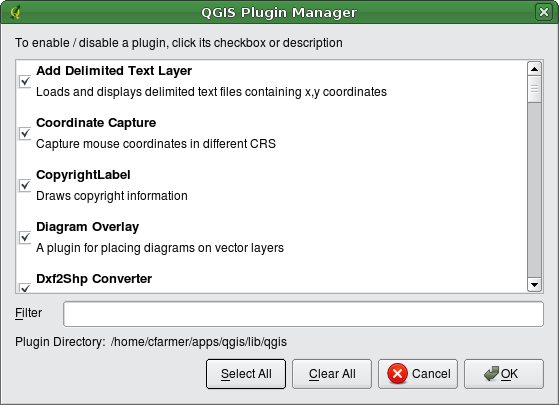
\includegraphics[clip=true, width=12cm]{pluginmanager}
   \caption{Plugin Manager \nixcaption}\label{fig:pluginmanager}\smallskip
\end{figure}

The \filename{Plugin Manager} lists all the available plugins and their
status (loaded or unloaded), including all core plugins and all external
plugins that have been installed and automatically activated using the
\filename{Python Plugin Installer} (see Section \ref{sec:external_plugins}).
Those plugins that are already loaded have a check mark to the left of
their name. Figure \ref{fig:pluginmanager} shows the Plugin Manager dialog.

To enable a particular plugin, click on the checkbox to the left of the
plugin name, and click \button{OK}. When you exit the application, a list
of loaded plugins is retained, and the next time you run QGIS these
plugins are automatically loaded.

\begin{Tip}\caption{\textsc{Crashing Plugins}}\index{crashes}
If you find that QGIS crashes on startup, a plugin may be at fault.
You can stop all plugins from loading by editing your stored settings file
(see \ref{subsec:gui_options} for location). Locate the plugins settings and
change all the plugin values to false to prevent them from loading.
\nix {For example, to prevent the Delimited text plugin from loading, the
entry in \$HOME/.config/QuantumGIS/qgis.conf on Linux should look like this:
\usertext{Add Delimited Text Layer=false}.}
\normalfont
Do this for each plugin in the [Plugins] section. You can then start QGIS
and add the plugins one at a time from the \filename{Plugin Manager} to
determine which plugin is causing the problem.
\end{Tip}

\subsection{Loading an external QGIS Plugin}\label{sec:load_external_plugin}

There is only one step required to integrate external plugins into QGIS:

\begin{itemize}[label=--]
\item Download an external plugin from a repository using the
\filename{Python Plugin Installer} (Section \ref{sec:python_plugin_installer}).
The new external plugin will be added to the list of available plugins in
the \filename{Plugin Manager} and is automatically loaded.
\end{itemize}

\subsection{Using the QGIS Python Plugin Installer}\index{plugins!installing}\label{sec:python_plugin_installer}
\index{plugins!Python Plugin Installer}\index{plugins!upgrading}

\begin{figure}[ht]
   \centering
   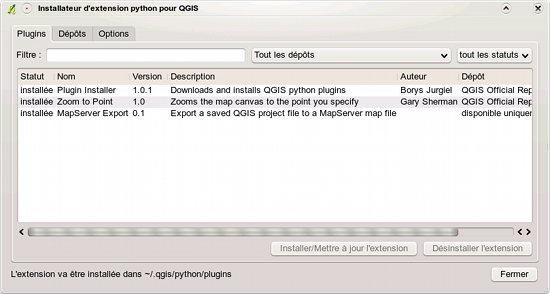
\includegraphics[clip=true, width=12cm]{plugininstaller}
   \caption{Installing external python plugins \nixcaption}\label{fig:plugininstaller}\smallskip
\end{figure}

In order to download and install an external Python plugin, click the
menu \mainmenuopt{Plugins} \arrow \dropmenuopttwo{plugin_installer}{Fetch
Python Plugins...}. The \filename{Plugin Installer} window will appear
(figure \ref{fig:plugininstaller}) with the tab \tab{Plugins}, containing
a list of all locally installed Python plugins, as well as plugins
available in remote repositories. Each plugin can be either:
\begin{itemize}[label=--]
\item \textbf{not installed} - this means the plugin is available in the repository, but is not installed yet. In order to install it, select the plugin from the list and click the \button{Install plugin} button.
\item \textbf{new} - this means that the plugin is newly available in the repository.
\item \textbf{installed} - this indicates that the plugin is already installed. If it is also available in any repository the \button{Reinstall plugin} button will be enabled. If the available version is older than the installed version, the \button{Downgrade plugin} button will appear instead.
\item \textbf{upgradeable} - this means that the plugin is installed, but there is an updated version available. In this case, the \button{Upgrade plugin} button will be enabled.
\item \textbf{invalid} - this means that the plugin is installed, but is unavailable or broken. The reason will be explained in the plugin description field.
\end{itemize}

\minisec{Plugins tab}

To install a plugin, select it from the list and click the \button{Install plugin}
button. The plugin is then activated and installed in its own directory.

\begin{itemize}[label=--]
\item \nix{Linux and other unices}:\\
./share/qgis/python/plugins \\
/home/\$USERNAME/.qgis/python/plugins
\item \osx{Mac OS X}:\\
./Contents/MacOS/share/qgis/python/plugins \\
/Users/\$USERNAME/.qgis/python/plugins
\item \win{Windows}:\\
C:\textbackslash Program Files\textbackslash QGIS\textbackslash
python\textbackslash plugins \\
C:\textbackslash Documents and Settings\textbackslash\$USERNAME\textbackslash
.qgis\textbackslash python\textbackslash plugins
\end{itemize}

If the installation is successful, a confirmation message will appear.

If the installation fails, the reason for the failure will be displayed
in a warning dialog. Most often, errors are the result of connection problems
and/or missing Python modules. In the former case you will likely need to
wait before trying the install again, in the latter case, you should install
the missing modules relevant to your operating system prior to using the
plugin. \nix{For Linux, most required modules should be available via a
package manager}. \win{For install instructions in Windows visit the module
home page}. If you are using a proxy, you may need to configure it under
\mainmenuopt{Edit} \arrow \dropmenuopttwo{mActionOptions}{Options} (Gnome, OSX)
or \mainmenuopt{Settings} \arrow \dropmenuopttwo{mActionOptions}{Options} (KDE, Windows)
on the \tab{Proxy} tab.

The \button{Uninstall plugin} button is enabled only if the selected plugin is installed and is not a core plugin. Note that if you have installed an update to a core plugin, you can uninstall this update with the \button{Uninstall plugin} and revert to the version shipped with Quantum GIS. This default version however, cannot be uninstalled.

\minisec{Repositories tab}

The second tab \tab{Repositories}, contains a list of plugin repositories available for the \filename{Plugin Installer}. By default, only the QGIS Official Repository is enabled. You can add several user-contributed repositories, including the central QGIS Contributed Repository and other external repositories by clicking the \button{Add 3rd party repositories} button. The added repositories contain a large number of useful plugins which are not maintained by the QGIS Development Team. As such, we cannot take any responsibility for them. You can also manage the repository list manually, that is add, remove, and edit the entries. Temporarily disabling a particular repository is possible by clicking the \button{Edit...} button.

\minisec{Options tab}

The \tab{Options} tab is where you can configure the settings of the \filename{Plugin Installer}. The \checkbox{Check for updates on startup} checkbox tells QGIS to automatically look for plugin updates and news. By default, if this feature is enabled all repositories listed and enabled in the \tab{Repositories} tab are checked for updates each time the program is started. The frequency of update checking can be adjusted using the dropdown menu, and may be adjusted from once a day right up to once a month. If a new plugin or update is available for one of the installed plugins, a notification will appear in the Status Bar. If the checkbox is disabled, looking for updates and news is performed only when the \filename{Plugin Installer} is manually launched from the menu.

Although the plugin installer update can handle ports different from 80, some internet
connections will cause problems when attempting to automatically check for updates.
In these cases, a \textit{Looking for new plugins...} indicator will
remain visible in the Status Bar during your entire QGIS session, and may cause a
program crash when exiting. In this case please disable the checkbox.

In addition, you may specify the type of plugins that are displayed by the \filename{Plugin Installer}. Under \textit{Allowed plugins}, you can specify whether you would like to:

\begin{itemize}[label=--]
\item Only show plugins from the official repository,
\item Show all plugins except those marked as experimental,
\item or Show all plugins, even those marked as experimental.
\end{itemize}

\begin{Tip}
 \caption{\textsc{Using experimental plugins}}
Experimental plugins are generally unsuitable for production use. These plugins are in the early stages of development, and should be considered 'incomplete' or 'proof of concept' tools. The QGIS development team does not recommend installing these plugins unless you intend to use them for
\end{Tip}

\section{Data Providers}\index{data providers}

Data Providers are "special" plugins that provides access to a data store.
By default, QGIS supports PostGIS layers and disk-based data stores supported by the GDAL/OGR library (Appendix \ref{appdx_ogr}).
A Data Provider plugin extends the ability of QGIS to use other data sources.

Data Provider plugins are registered automatically by QGIS at startup.
They are not managed by the Plugin Manager but used behind the scenes when a data type is added as a layer in QGIS.

\FloatBarrier
